\documentclass{article}
\usepackage[utf8]{inputenc}
\usepackage{amsmath}
\usepackage{amsthm}
\usepackage{graphicx}
\usepackage{hyperref}
\usepackage{geometry}
\geometry{a4paper, portrait, margin=1in}

\usepackage{geometry}
\geometry{a4paper, portrait, margin=1in}

\theoremstyle{plain}
\newtheorem{thm}{Theorem}

\theoremstyle{definition}
\newtheorem{defn}{Definition} % definition numbers are dependent on theorem numbers
\newtheorem{exmp}{Example} % same for example numbers

\title{Computer Networks (UE18CS301)\\
 \large Unit 2
 }
\author{Aronya Baksy}
\date{August 2020}

\begin{document}
\maketitle

\section{Application Layer}
\subsection{Principles of Network Applications}
\begin{itemize}
    \item Network Applications are programs that run on different host systems and communicate with each other along a network.
    
    \item Network applications are written at an abstract level, without the hardware details of link-layer devices (switches) or network-layer devices (routers). 
    
    \item These low level details are presented to the application layer only as an abstraction.
\end{itemize}

\subsection{Network Application Architectures}
\subsubsection{Client-Server Architecture}
\begin{itemize}
    \item There is an always-on host machine called the \textbf{server}, which services requests from resources from many machines. A machine that makes a request is called a \textbf{client}.
    
    \item Clients do not directly communicate with each other. They always communicate via the server.
    
    \item Since the server has a fixed address called the IP Address, and it is always on, the server is always reachable by any client. 
    
    \item In order to avoid a single server getting overwhelmed by large volume of client requests,\textbf{data centers} containing large number of servers aggregated together are used by large content providers. 
    
    \item Such companies must pay bandwidth and interconnection costs, apart from maintenance and power costs for upkeep of these data centers. 
\end{itemize}

\subsubsection{Peer-to-Peer Architecture (P2P)}
\begin{itemize}
    \item In a P2P architecture, communication takes place between pairs of intermittently connected hosts (aka \textbf{peers}). 
    
    \item These peer machines are not large servers but common desktop/laptop machines owned by daily users. 
    
    \item P2P architectures have the advantage of self scalability as peers are capable of requesting and adding services to the network at the same time.
    
    \item P2P architecture has the following disadvantages:
    \begin{itemize}
        \item Not ISP friendly as most ISPs are optimized for more volume of downstream traffic than upstream (aka asymmetric usage). But P2P applications shift a large volume of upstream traffic from servers to the local ISPs.
        
        \item Not secure as they are open and highly distributed.
        
        \item Not enough incentive for users to donate their own bandwidth and power to offer service to other peers.
    \end{itemize}
\end{itemize}

\subsection{Process Communication}
\begin{itemize}
    \item Processes are labelled as client and server based on the one who initiated the communication session (client), and the one who is waiting to be contacted to begin the session (server). 
    
    \item The \textbf{socket} is the interface between an application running on the application layer, and the rest of the TCP/IP layers below it. A socket is a combination of the IP Address and the Port Number. 
    
    \item The socket is a software interface that acts like a gateway for processes to communicate over a network. 
    
\end{itemize}
\begin{figure}[!h]
    \centering
    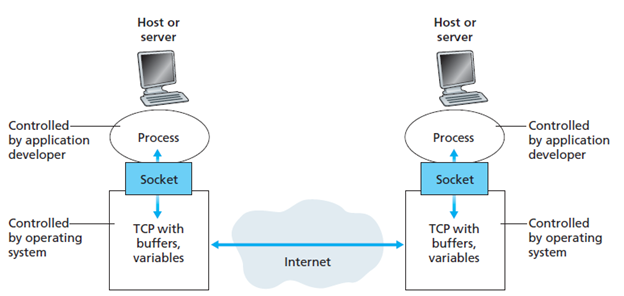
\includegraphics[scale=0.9]{cn1.png}
    \caption{Socket illustration}
    \label{fig:my_label}
\end{figure}

\begin{itemize}
    \item The IP address of a host machine identifies it uniquely in a network. 
    
    \item The \textbf{port number} identifies a particular application or process within a host machine. 
    
    \item The port number is used to distinguish between multiple different network applications running on a single host machine. 
    
    \item Some common port numbers are: 80 for HTTP, 443 for HTTPS, 20 and 21 for FTP, and either 25, 465/587 or 2525 for SMTP.
    
    \item The IP Address is a 32 bit integer, while the port number is a 16 bit integer value (port numbers range from 0 to 65535).
    
    \item Port numbers 0 to 1023 are known as \textit{well-known ports} allocated to server services by the IANA, ports 1024 to 49151 are \textit{registered ports} (semi reserved, services) and ports 49151 onwards are used by \textit{client} programs. 
\end{itemize}

\section{Transport Layer Services}
The following are some of the services that are available to the application layer from the transport layer
\begin{itemize}
    \item \textbf{Reliable Data Transfer}: Guarantee that no data will be lost or will arrive out of sequence at the receiver from the sender. Some applications do not require this (eg: audio/video streaming)
    
    \item \textbf{Throughput}: Guarantee of a fixed throughput across a link, important for some throughput sensitive applications (eg: internet telephony).
    
    \item \textbf{Timing}: Guarantee of delay between server and receiver being less than or equal to some fixed value, important for real-time applications like telephony, online gaming etc.
    
    \item \textbf{Security}: Services like encryption allow for confidentiality between sender and receiver, along with other security services like data integrity checking and end-point authentication.
\end{itemize}

\subsection{Transmission Control Protocol (TCP)}
\begin{itemize}
    \item TCP is a \textbf{connection-oriented} protocol. This means that before any actual data is sent between 2 host machines, they must go through a \textbf{handshaking} process first.
    
    \item The objective of this handshaking is to set up the validity of the connection, and it consists of 3 packets sent: client sends SYN to server, server sends SYN/ACK to client, and client responds with ACK.
    
    \item TCP also implements \textbf{reliable data transfer}. TCP can be relied on to transmit data from one host to another in correct order with zero loss. 
    
    \item TCP also includes additional services for \textbf{congestion control} and \textbf{flow control} to manage TCP traffic along busy networks. 
\end{itemize}

\subsection{User Datagram Protocol (UDP)}
\begin{itemize}
    \item UDP is a connection-less protocol, meaning that there is no initial set up of a connection between two communicating processes before the actual data transfer
    
    \item UDP does not provide reliable data transfer, and it also does not provide services like congestion control.
    
    \item UDP offers the advantage of greater speed than TCP, which is useful for real-time network applications (eg: video streaming, online conferencing etc.).
\end{itemize}

\section{Application Layer Protocols}
The following are defined as part of any application layer protocol.
\begin{itemize}
    \item Types of messages to be exchanged (eg: request and response)
    
    \item Message syntax (eg: fields and how fields are delineated)
    
    \item Message semantics (meaning of all the fields in the message)
    
    \item Rules to determine when and how messages are sent and responded to.
\end{itemize}
Application layer protocols such as HTTP, SMTP, FTP and proprietary protocols like Skype etc. are one important component of all network applications. 

\section{Hypertext Transfer Protocol (HTTP)}
\begin{itemize}
    \item HTTP is the application-layer protocol that is at the heart of the world wide web. 
    
    \item A web page consists of different \textbf{objects} (HTML files, images, documents, Java applets etc.). Every web page on the internet has a \textbf{base HTML} file and the associated resources with it. 
    
    \item Every resource has its own unique Uniform Resource Locator (URL). 
    
    \item The client requests for HTTP objects, receives them from server and processes them (displaying or otherwise).
    
    \item The server listens for requests and responds to them by sending the appropriate message.
    
    \item The HTTP protocol is defined in RFC 1945 (version 1.0) and RFC 2616 (version 1.1). 
\end{itemize}

\subsection{Overview of HTTP}
\begin{itemize}
    \item HTTP uses TCP as its underlying transport layer protocol. 
    
    \item First, the client initiates a TCP connection with the server. Once the connection is established, client and server communicate via their respective socket interfaces. 
    
    \item The client sends requests and receives responses through its socket interface, while the server receives requests and sends responses through its socket interface.
    
    \item Reliable data transfer and the transport layer services are maintained by the TCP protocol on the transport layer, and are not of concern to HTTP.
    
    \item HTTP is a \textbf{stateless} protocol, in that a server does not maintain any information about any past transactions with a client.
    
    \item Whenever a client requests for a resource from a server that has been previously requested for the same resource by the same client, a \textbf{new connection} will be opened that does not contain any information about past connections.
    
    \item The advantage of a stateless protocol are as follows:
    \begin{itemize}
        \item If either client or server fails, then the state that each machine sees may differ, hence causing conflict when the connection is to be resumed.
        
        \item No need for dynamic memory allocation when connection is starting and ongoing, and no need for any cleanup when a connection terminates/fails.
    \end{itemize}

\end{itemize}
\begin{figure}
    \centering
    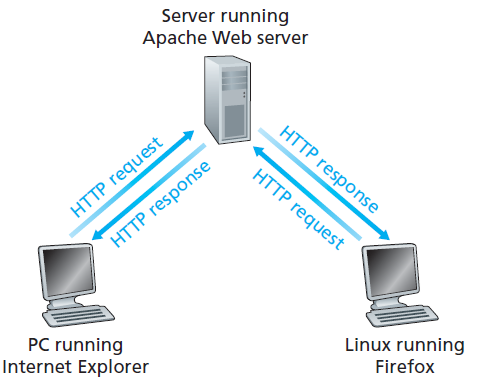
\includegraphics[scale=0.6]{cn2.png}
    \caption{Request-Response Behaviour of HTTP}
    \label{fig:my_label_2}
\end{figure}

\subsection{Persistent and Non-Persistent HTTP}
\begin{itemize}
    \item \textbf{Non persistent connections} describe the situation where each request-response pair between 2 hosts takes place over a separate TCP connection
    
    \item Only one object can be sent along a non-persistent connection before it is closed. 
    
    \item The steps in establishing a non-persistent connection are:
    
    \begin{itemize}
        \item Client initiates a connection on Port 80 to the server. The server starts up a socket associated with this connection
        
        \item Client sends HTTP request to server containing the path of the requested resource within the server
        
        \item The server receives the request, locates the resource requested, encapsulates it within the response message and sends it.
        
        \item Client receives the response and closes the TCP connection. Client processes the response and handles the object that was sent back.
    \end{itemize}
    
    \item The entire response time for a single object over a Non-Persistent connection is
    \begin{equation*}
        HTTP\text{ }Response\text{ }Time = 2 \times RTT + Obj\text{ }Transfer\text{ }Time
    \end{equation*}
\end{itemize}
\begin{figure}
    \centering
    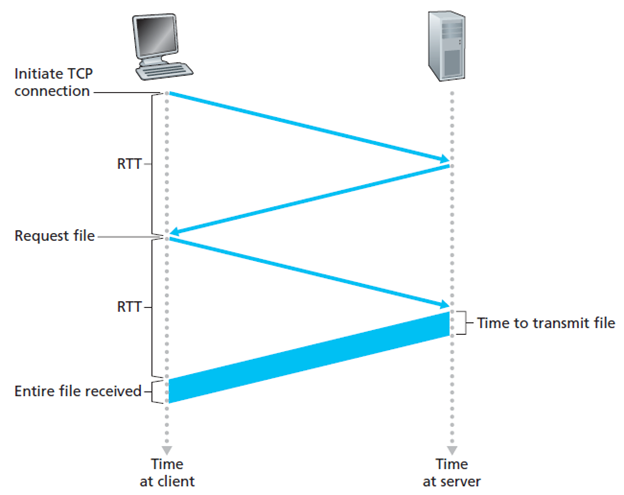
\includegraphics[scale=0.6]{cn3.png}
    \caption{Non-persistent HTTP connection}
    \label{fig:my_label_3}
\end{figure}
\begin{itemize}
    \item Non persistent connections suffer from increased overhead on the server end to open and close multiple TCP connections, and increased time for object transmission (2 RTTs).
    
    \item In a \textbf{persistent connection}, the connection is kept open even after the server sends a response
    
    \item All subsequent communication between server and client can take place over the same connection.
    
    \item These requests for objects can be made back-to-back, without waiting for replies to pending requests (pipelining).
    
    \item When the server receives the back-to-back requests, it sends the objects back-to-back.
    
    \item Response time is cut in half in persistent connection compared to non-persistent.
\end{itemize}

\subsection{HTTP Message Format}
\subsubsection{HTTP Request Format}
\begin{itemize}
    \item The first line of HTTP request is called the request line. It is followed by the header lines that contain information about the request, and the entity body.
    
    \item The request line contains information about the type of request (GET, POST, PUT, HEAD or DELETE), the location of the requested resource on the server, and the version of HTTP used (1.0 or 1.1). It is used by Web caches.
    
    \item The \texttt{Connection} header field defines whether the connection is persistent (\texttt{Keep-Alive}) or non-persistent (\texttt{close}). 
    
    \item The entity body is empty for GET requests, but contains information when used with POST method. 
    
    \item The POST method is used to securely fill forms without exposing user information. The HEAD method is used when the client only wants the HTTP header in response and not any actual content. The PUT and DELETE methods are used to store and remove files to/from a certain directory in the web server.
\end{itemize}
\begin{figure}[!h]
    \centering
    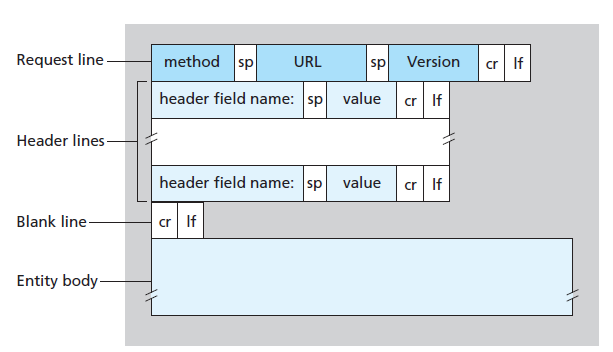
\includegraphics[scale=0.8]{cn4.png}
    \caption{HTTP Request Message Format}
    \label{fig:my_label_4}
\end{figure}
\subsubsection{HTTP Response Format}
\begin{itemize}
    \item The HTTP response consists of a status line, followed by header lines, then a blank line and finally the resource content (the entity body). 
    
    \item The status line contains the HTTP version (1.0 or 1.1), the status code (a 3 digit number) and the English phrase associated with that code. 
    
    \item Some important status codes are \texttt{200 OK, 301 Moved Permanently, 304 Not Modified, 400 Bad Request, 404 Not Found} and \texttt{501 HTTP Version Not Supported}. 
\end{itemize}

\begin{figure}[!h]
    \centering
    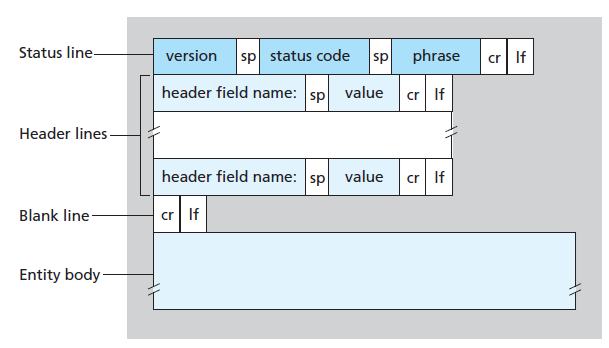
\includegraphics[scale=0.8]{cn5.png}
    \caption{HTTP Response Message Format}
    \label{fig:my_label_5}
\end{figure}

\subsection{HTTPS}
\begin{itemize}
    \item HTTPS stands for HTTP Secure or HTTP over Secure Socket Layer (SSL). It integrates HTTP with an encryption standard that is bidirectional (client to server and server to client are both encrypted communications).
    
    \item HTTPS uses port number 443 as its standard port. 
    
    \item TLS (Transport Layer Security) is the most recent encryption standard that is used by HTTPS (because SSL is now deprecated). The most recent version is TLS 1.3 (RFC 8446).
    
    \item All TLS connections have the following properties:
    \begin{enumerate}
        \item Connection is \textbf{secure} as the key is based on a \textit{shared secret} that is negotiated between client and server before any data is transmitted, at the start of the session. This negotiation is secure (the key cannot be found even by an attacker in the middle of the connection) and reliable (no attacker can modify this communication without being detected). 
        
        \item The identity of the two parties can be \textbf{authenticated} using public key cryptography. This authentication can be made optional, but is generally required for at least one party (server)
        
        \item Connection is \textbf{reliable} as message integrity is checked using a \textit{message authentication code} to prevent loss or alteration of data. 
    \end{enumerate}
    
    \item TLS and SSL rely on \textbf{certificates} issued by trusted third parties that certifies the ownership of a public key by the subject of the certificate. 
    
    \item The following steps are involved in a HTTPS communication:
    \begin{enumerate}
        \item Browser requests secure pages from server
        
        \item Server sends its public key with its SSL certificate (digitally signed by a third party – CA)
        
        \item On receipt of certificate, browser verifies issuer’s digital signature. (This is commonly denoted by green padlock key symbol in the browser).
        
        \item Browser creates a symmetric key (shared key), keeps one and gives a copy to server. This symmetric shared key is encrypted using server’s public key before sending.
        
        \item On receipt of encrypted secret key, server decrypts it using its private key and gets browser’s secret symmetric key.
    \end{enumerate}
    
    \item Asymmetric encryption is used to verify identity of the owner and its public key, hence establishing trust between client and server. 
    
    \item Symmetric encryption is used for actual data transfer. 
\end{itemize}

\subsection{Cookies}
\begin{itemize}
    \item Even though HTTP is a stateless protocol, cookies are one method for servers to maintain state information about clients.
    
    \item Cookie technology has 4 components: HTTP Request header, HTTP Response header, the cookie file kept on client end system and managed by the user's browser, and the back end database at the server end. 
    
    \item Cookie information is exchanged over request and response headers.
    
    \item The identification number for a user can be linked to a database on the server side that contains all the information of that user. This can be used to quickly offer personal experience to the user
    
    \item This is used by e-commerce websites like Amazon and eBay to deliver their shopping cart service and personalized recommendations.
\end{itemize}
\begin{figure}[!ht]
    \centering
    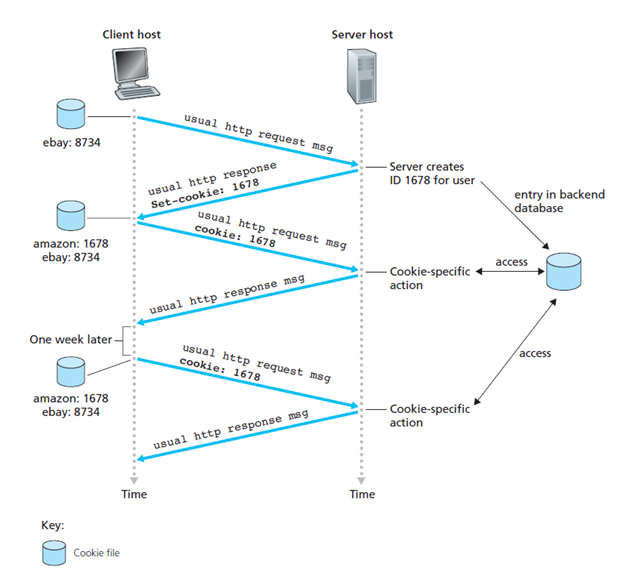
\includegraphics[scale=0.7]{cn6.png}
    \caption{Maintaining user state with cookies}
    \label{fig:my_label_6}
\end{figure}

\subsection{Web Caching}
Web cache is a server in between client and server that services requests for popular resources much faster than the actual server. 
\begin{itemize}
    \item The client opens TCP connection to the web cache and sends HTTP request to it.
    
    \item Cache checks if a copy of the resource is stored, If yes then it is sent on the response
    
    \item If not, the cache sends an HTTP request to the origin server for the resource, receives a response, and stores a copy of the object from the origin server in its storage. Then that object is sent back to the client.
    
    \item Cache acts as server for the client side, and as a client to the origin server. They are installed by the ISP.
    
    \item Cache reduces the traffic intensity on access link between institutional network and public network, as well as reducing average response times for HTTP requests. 
\end{itemize}

\section{Domain Name System (DNS)}
\begin{itemize}
    \item The DNS offers the service of translating human-readable hostnames to IP Addresses that can be used to locate hosts.
    
    \item DNS is an application-layer protocol that relies on a \textbf{distributed network} of \textbf{DNS Servers} to provide this service. 
\end{itemize}

\subsection{DNS Services}
\begin{itemize}
    \item \textbf{Host Aliasing}: Mapping shorter hostnames like \texttt{enterprise.com} and \texttt{www.enterprise.com} to larger actual hostnames like \texttt{relay1.west-coast.enterprise.com} (aka the \textit{canonical hostname}). 
    
    \item \textbf{Mail Server Aliasing}: Translation between canonical mail server host names and user level mnemonic mail server host names. The MX record in the DNS header allows the mail server and web server to share the same hostname.
    
    \item \textbf{Load Distribution}: If a busy website has multiple servers, and the DNS is aware of the IP Addresses of all these servers, then requests to that website are rotated between all the servers to ensure uniform distribution between all the servers. \\
    This is done by the DNS changing the order of the table of IP Addresses that are sent to the client. 
\end{itemize}
\subsection{Working of DNS}
\begin{itemize}
    \item DNS consists of the following hierarchy of distributed servers: (top to bottom)
    \begin{itemize}
        \item \textbf{Root DNS Servers}: There are 13 IP Addresses associated with root level server networks. Each IP Address leads to a network of replicated root level DNS Servers. 
        
        \item \textbf{Top Level Domain (TLD) Servers}: The DNS servers for top level domains like com, edu as well as country level TLDs like in, pk, fr, us, jp etc.
        
        \item \textbf{Authoritative DNS Servers}: Every pyblicly accessible host provides a public DNS record on the authoritative servers. Large institutions/companies maintain their own Authoritative servers, and smaller ones rent this service from a provider. 
    \end{itemize}
    
    \item The \textbf{Local DNS server} does not belong to this hierarchy but is very important. It acts as a web cache or a proxy server to the client machines. 
    
    \item The local DNS server is installed by an ISP, and when a host connects to this ISP's network, it is provided with a list of IP Addresses of the local DNS servers (done using DHCP).
    
    \item The local DNS server forwards a query from host to the main DNS hierarchy.
\end{itemize}
\begin{figure}
    \centering
    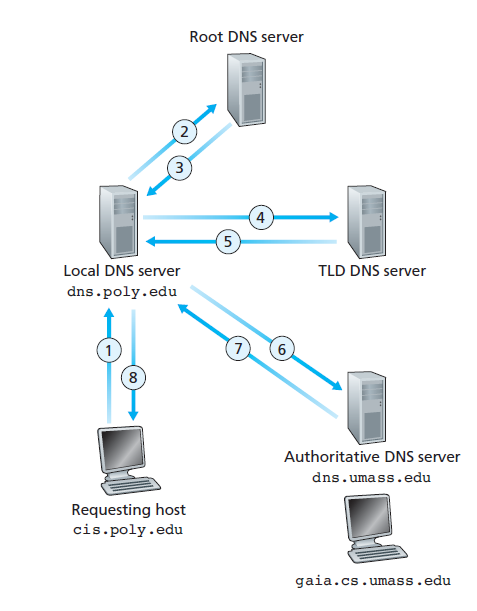
\includegraphics[scale=0.7]{cn7.png}
    \caption{Working of DNS}
    \label{fig:my_label_7}
\end{figure}
\begin{itemize}
    \item Queries to DNS servers can be iterative or recursive.
    
    \item The query from client to the Local DNS server is a recursive query as the query asks the local DNS server to obtain the mapping on its behalf.
    
    \item The other queries are all iterative as the local DNS directly receives the reply for its requests.
    
    \item DNS queries can be entirely recursive or entirely iterative, but in the real world the pattern below is most common. 
\end{itemize}

\subsection{DNS Caching}
\begin{itemize}
    \item Whenever a DNS server receives a response to a query, it can store this response in its own memory.
    
    \item The next time a request is received for this particular mapping, it can respond with the IP Address despite not being an authoritative DNS server for that host. 
    
    \item The cache is cleared every 2 days as mappings between hostnames and IP Addresses are not permanent. 
\end{itemize}

\subsection{DNS Records and Messages}
\begin{itemize}
    \item A DNS record consists of a 4-tuple \texttt{(Name, Value, Type, TTL)}
    
    \begin{itemize}
        \item If \texttt{Type=A}, then \texttt{Name} is the hostname and \texttt{Value} is the IP Address for that hostname. 
        
        \item If \texttt{Type=NS}, then \texttt{Name} is a domain and \texttt{Value} is the hostname of an authoritative server that knows the IP Addresses of all the hosts in that domain.
        
        \item If \texttt{Type=CNAME}, then \texttt{Name} is an alias hostname and \texttt{Value} is the canonical hostname.
        
        \item If \texttt{Type=MX}, then \texttt{Name} is an alias hostname and \texttt{Value} is the canonical hostname of a mail server. 
    \end{itemize}
    
    \item The \texttt{CNAME} and \texttt{MX} types allow mail and web servers to have the same alias hostname. If mail server's canonical hostname is required, then the MX record is queried, and CNAME is queried if web server's canonical hostname is required. 
\end{itemize}

\subsubsection{DNS Message Format}
\begin{itemize}
    \item The first 12 bytes (96 bits) makes up the header section
    
    \item The header section consists of a 16-bit query ID, 16-bit flags field, and the number of question, answer, authority and additional records in the message. 
    
    \item Some flags are:
    
    \begin{itemize}
        \item \textit{Query(0)/reply(1) flag}, indicates whether message is query or reply
        
        \item \textit{Authoritative flag} is set in response if the server sending the response is authoritative
        
        \item \textit{Recursion desired}, and \textit{recursion supported} flags
    \end{itemize}
    
    \item The question section contains query information, with the name field and the type of query.
    
    \item Answer section in a reply message consists of the resource records pulled from the server. This can have more than 1 record as one hostname can have multiple IP Addresses (replicated servers).
    
    \item Authority section contains info about other authoritative servers
    
    \item The additional section contains other helpful records. For example, the answer field in a reply to an MX query contains a resource record providing the canonical hostname of a mail server. The additional section contains a Type A record providing the IP address for the canonical hostname of the mail server.
\end{itemize}

\section{Peer to Peer Applications}
\subsection{BitTorrent Protocol}
\begin{itemize}
    \item The collection of all peers participating in file distribution is called the \textit{torrent}. Peers in a torrent download \textbf{chunks} of a file from each other (typical chunk size is 256 kB). 
    
    \item Peers may leave once the file is downloaded entirely (selfish) or continue to supply chunks to other peers in the torrent (altruistic).
    
    \item In the network of peers, one node is designated as a \textbf{tracker}. Tracker tracks all the nodes that are in the torrent. Before joining the torrent a peer must inform the tracker of this. 
    
    \item When a new peer joins, the tracker randomly selects 50 nodes in the torrent and sends their IP Addresses to the new node. The new node establishes concurrent TCP connections with all these nodes. The nodes with which TCP connection is successfully established by the new node are called the \textbf{neighbouring peers}. 
    
    \item Periodically, a peer asks its neighbouring peers for a list of chunks they have. Given these lists, the peer can ask its neighbours for the chunks it does not have using the TCP connection.
    
    \item The \textbf{rarest first} protocol is used to determine the order of chunk gathering. In this protocol, the least frequently stored chunk is requested first by the peer. Over time, this equalizes the number of copies of each chunk stored accross the torrent. 
    
    \item When responding to requests for chunks, a peer will give priority to the 4 peers that send it chunks at the \textbf{maximum rate}. The peer sends these 4 replies in return. These 4 peers are said to be \textbf{unchoked}.
    
    \item The top 4 peers are updated every 10 seconds by checking the transfer rates. 
    
    \item In addition to the 4 unchoked peers, one additional neighbour is randomly chosen and the peer sends it chunks. This is called the \textbf{optimistically unchoked} peer. A new randomly chosen peer is optimistically unchoked every 30 seconds. 
    
    \item If the two peers are satisfied with the trading, they will put each other in their top four lists and continue trading with each other until one of the peers finds a better partner. 
    
    \item The effect is that peers capable of uploading at compatible rates tend to find each other. 
    
    \item The random neighbor selection also allows new peers to get chunks, so that they can have something to trade.
\end{itemize}

\subsection{Distribution Time Calculation}
The distribution time is defined as the length of time taken to transfer a copy of the file to all the machines on the network.
\subsubsection{Client-Server Architecture}
\begin{itemize}
    \item Number of clients in the network is $N$ and file size is $F$ bits.
    
    \item The upload rate of server's access link is $u_s$, the upload rate of the client access links is $u_i$ for the $i^{th}$ client, and the download rate of the client access links is $d_i$ for the $i^{th}$ client.
    
    \item Initially only the server has the file. The time taken to upload $N$ copies of the file is $\frac{NF}{u_s}$
    
    \item The time taken for the clients to receive the file is limited by the one with the smallest download rate $d_i$. Let $d_{min} = min(d_1, d_2, .., d_N)$. Then the time taken to download the file is $\frac{F}{d_{min}}$. 
    
    \item The distribution time can be calculated as
    \begin{equation}
        d_{CS} = max \left \{ \frac{NF}{u_s}, \frac{F}{d_{min}}  \right \}
    \end{equation}
\end{itemize}

\subsubsection{Peer to Peer Architecture}
\begin{itemize}
    \item The server must send one copy of the file into the access network. This is done in time $\frac{F}{u_s}$.
    
    \item The peer with the lowest download rate will get a copy of the file from the network in time $\frac{F}{d_{min}}$.
    
    \item The total upload capacity of the system $u_{total} = u_s + u_1 + u_2 + .. + u_n$. The system must deliver (upload) F bits to each of the N peers, thus delivering a total of NF bits. This cannot be done at a rate faster than $u_{total}$. Hence the distribution time is also at least $\frac{NF}{u_{total}}$
    
    \item Hence the distribution time is given by
    \begin{equation}
        d_{P2P} = max \left \{ \frac{F}{u_s}, \frac{F}{d_{min}}, \frac{NF}{u_{total}}  \right  \}
    \end{equation}
\end{itemize}

\section{Other Application Layer Protocols}

\subsection{File Transfer Protocol (FTP)}
\begin{itemize}
    \item Uses TCP to exchange large files over internet. FTP uses two parallel TCP connections for a single file exchange, called the \textbf{data connection} (port 20) and the \textbf{control connection}(port 21). 
    
    \item File manipulation (rename, move, put, get) as well as identification (user ID, password) information is sent over the control connection while the actual file contents are exchanged over the data connection. 
\end{itemize}

\subsection{Simple Mail Transfer Protocol (SMTP)}
\begin{itemize}
    \item It is an application layer protocol or electronic mail transfer. It uses TCP port 25.
    
    \item All SMTP communication are secured using SSL or TLS.
    
    \item SMTP servers run on a centralized mail server (like gmail.com or yahoo.com). The clients open TCP connections to these mail servers.
    
    \item Message from client enters client's mailbox located in client server. From the client mailbox, it enters the central message queue of the client mail server. From here, the message is sent by TCP to the destination mail server's message queue.
    
    \item From the destination message queue, the message is routed to the destination user's individual mailbox. The destination user can now access their mailbox at their convenience. 
\end{itemize}

\subsection{Dynamic Host Configuration Protocol (DHCP)}
\begin{itemize}
    \item It is an application layer service that is used to assign IP Addresses to hosts on a network dynamically. 
    
    \item For server it runs on port 67, on client it runs on port 68. 
    
    \item DHCP uses a client-server model, and it runs on a sequence of discovery, offer, request and ACK. 
    
    \item Aside from the IP Address, DHCP assigns the subnet mask, the local DNS server, and the default gateway. 
\end{itemize}

\subsection{Simple Network Management Protocol (SNMP)}
\begin{itemize}
    
    \item Exchange of management information between network devices is handled by SNMP protocol
    
    \item SNMP runs on ports 161 and 162. It uses both TCP and UDP. 
    
    \item SNMP consists of the following components:
    \begin{itemize}
        \item \textit{SNMP Manager}: Oversees all managed devices.
        
        \item \textit{Managed Devices}: Host machines, routers, link-layer switches that run agent software. 
        
        \item \textit{SNMP Agents}: Software installed in all managed devices. 
        
        \item \textit{Management Info Base}: Store details of managed devices. One per device. 
    \end{itemize}
\end{itemize}

\subsection{Remote Access: Telnet and SSH}
\begin{itemize}
    \item Telnet and SSH are remote access protocols that allow, for example, network admins to remotely monitor the state of devices that are connected to a network. 
    
    \item Telnet uses port 23 of TCP, while SSH uses port 22. Telnet uses TCP exclusively while SSH uses both TCP and UDP. 
    
    \item Telnet transfers all data as plain text, while SSH transfers data in encrypted form using \textit{public key} encryption. 
    
    \item Telnet is susceptible to middle man attacks where hackers listen to the telnet connection and get the user's authentication information 
\end{itemize}
\end{document}